\documentclass[reprint, amsmath, amssymb, aps, onecolumn, superscriptaddress, floatfix, 10pt]{revtex4-2}
\usepackage{xcolor}
\usepackage{color}
\usepackage{tikz}
\usepackage{tikz-cd}
\usepackage{pgfplots}
\usepgfplotslibrary{groupplots}
\pgfplotsset{compat=1.18}

\newcommand{\wstar}{\ensuremath{\boldsymbol{\theta}_0}}

\newcommand{\what}{\ensuremath{\hat{\boldsymbol{\theta}}}}

\begin{document}

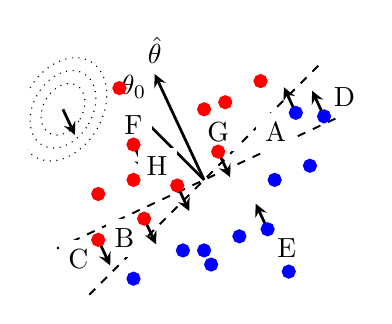
\begin{tikzpicture}[scale=1.0]
\begin{axis}[
        width=0.5\textwidth,
        height=0.5\textwidth,
        xmin=-2.5, xmax=2.5,
        ymin=-2.5, ymax=2.5,
        hide axis,
        domain=-2.5:2.5,
        xtick=\empty, 
        ytick=\empty,
        grid=major
    ]
    % definitions for the teacher vector B and the student vector A
    \pgfmathsetmacro\Bx{-1}
    \pgfmathsetmacro\By{1}
    \pgfmathsetmacro\NormB{sqrt(\Bx*\Bx + \By*\By)}
    \pgfmathsetmacro\UnitBx{\Bx / \NormB}
    \pgfmathsetmacro\UnitBy{\By / \NormB}

    \pgfmathsetmacro\Cx{-0.7}
    \pgfmathsetmacro\Cy{1.5}
    \pgfmathsetmacro\NormC{sqrt(\Cx*\Cx + \Cy*\Cy)}
    \pgfmathsetmacro\UnitCx{\Cx / \NormC}
    \pgfmathsetmacro\UnitCy{\Cy / \NormC}

    % radius of the circle boundary line
    \pgfmathsetmacro\R{2.3}
    \pgfmathsetmacro\epsfigure{0.4}

    \draw[-stealth, line width=1pt] (0,0) -- (\Bx, \By) node[above] {$\wstar$};
    \draw[-stealth, line width=1pt] (0,0) -- (\Cx, \Cy) node[above] {$\what$};

    \pgfmathsetmacro\slopeB{- \Bx/\By}
    \pgfmathsetmacro\slopeC{- \Cx/\Cy}

    \pgfmathsetmacro\BoundaryB{abs(\R * cos(atan(\slopeB)))}
    \pgfmathsetmacro\BoundaryC{abs(\R * cos(atan(\slopeC)))}

    \addplot[domain=-\BoundaryB:\BoundaryB, dashed, black, line width=0.7]{\slopeB * x };
    \addplot[domain=-\BoundaryC:\BoundaryC, dashed, black, line width=0.7]{\slopeC * x };

    % add the points that are going to be used for the explanation
    \pgfmathsetmacro\PointOneX{1.3}
    \pgfmathsetmacro\PointOneY{0.95}

    \pgfmathsetmacro\PointTwoX{-0.85}
    \pgfmathsetmacro\PointTwoY{-0.55}

    \pgfmathsetmacro\PointThreeX{-1.5}
    \pgfmathsetmacro\PointThreeY{-0.85}

    \pgfmathsetmacro\PointFourX{1.7}
    \pgfmathsetmacro\PointFourY{0.9}

    \pgfmathsetmacro\PointFiveX{0.9}
    \pgfmathsetmacro\PointFiveY{-0.7}

    \pgfmathsetmacro\PointSixX{-1.0}
    \pgfmathsetmacro\PointSixY{0.5}

    \pgfmathsetmacro\PointSevenX{0.2}
    \pgfmathsetmacro\PointSevenY{0.4}

    \pgfmathsetmacro\PointEightX{-0.38}
    \pgfmathsetmacro\PointEightY{-0.08}

    % drawing the points
    \addplot [only marks, mark=oplus, mark options={line width=2pt}, mark size=1.5pt, color=blue] coordinates {(\PointOneX,\PointOneY)} node[anchor=north east,black,fill=white] {A};
    \draw[-stealth, line width=1pt] (\PointOneX,\PointOneY) -- (\PointOneX + \epsfigure * \UnitCx,\PointOneY + \epsfigure * \UnitCy);

    \addplot [only marks, mark=oplus, mark options={line width=2pt}, mark size=1.5pt, color=red] coordinates {(\PointTwoX,\PointTwoY)} node[anchor=north east, black, fill=white] {B};
    \draw[-stealth, line width=1pt] (\PointTwoX,\PointTwoY) -- (\PointTwoX - \epsfigure * \UnitCx,\PointTwoY - \epsfigure * \UnitCy);

    \addplot [only marks, mark=oplus, mark options={line width=2pt}, mark size=1.5pt, color=red] coordinates {(\PointThreeX,\PointThreeY)} node[anchor=north east, black, fill=white] {C};
    \draw[-stealth, line width=1pt] (\PointThreeX,\PointThreeY) -- (\PointThreeX - \epsfigure * \UnitCx,\PointThreeY - \epsfigure * \UnitCy);

    \addplot [only marks, mark=oplus, mark options={line width=2pt}, mark size=1.5pt, color=blue] coordinates {(\PointFourX,\PointFourY)} node[anchor=south west,black,fill=white] {D};
    \draw[-stealth, line width=1pt] (\PointFourX,\PointFourY) -- (\PointFourX + \epsfigure * \UnitCx,\PointFourY + \epsfigure * \UnitCy);

    \addplot [only marks, mark=oplus, mark options={line width=2pt}, mark size=1.5pt, color=blue] coordinates {(\PointFiveX,\PointFiveY)} node[anchor=north west,black,fill=white] {E};
    \draw[-stealth, line width=1pt] (\PointFiveX,\PointFiveY) -- (\PointFiveX + \epsfigure * \UnitCx,\PointFiveY + \epsfigure * \UnitCy);

    \addplot [only marks, mark=oplus, mark options={line width=2pt}, mark size=1.5pt, color=red] coordinates {(\PointSixX,\PointSixY)} node[above,black,fill=white] {F};
    \draw[-stealth, line width=1pt] (\PointSixX,\PointSixY) -- (\PointSixX - \epsfigure * \UnitCx,\PointSixY - \epsfigure * \UnitCy);

    \addplot [only marks, mark=oplus, mark options={line width=2pt}, mark size=1.5pt, color=red] coordinates {(\PointSevenX,\PointSevenY)} node[above,black,fill=white] {G};
    \draw[-stealth, line width=1pt] (\PointSevenX,\PointSevenY) -- (\PointSevenX - \epsfigure * \UnitCx,\PointSevenY - \epsfigure * \UnitCy);

    \addplot [only marks, mark=oplus, mark options={line width=2pt}, mark size=1.5pt, color=red] coordinates {(\PointEightX,\PointEightY)} node[anchor=south east,black,fill=white] {H};
    \draw[-stealth, line width=1pt] (\PointEightX,\PointEightY) -- (\PointEightX - \epsfigure * \UnitCx,\PointEightY - \epsfigure * \UnitCy);


    % drawing additional points REDS
    \addplot [only marks, mark=oplus, mark options={line width=2pt}, mark size=1.5pt, color=red] coordinates {(-1.2,1.3)};
    \addplot [only marks, mark=oplus, mark options={line width=2pt}, mark size=1.5pt, color=red] coordinates {(0.0,1)};
    \addplot [only marks, mark=oplus, mark options={line width=2pt}, mark size=1.5pt, color=red] coordinates {(-1.0,0.0)};
    \addplot [only marks, mark=oplus, mark options={line width=2pt}, mark size=1.5pt, color=red] coordinates {(-1.5,-0.2)};
    \addplot [only marks, mark=oplus, mark options={line width=2pt}, mark size=1.5pt, color=red] coordinates {(0.8,1.4)};
    \addplot [only marks, mark=oplus, mark options={line width=2pt}, mark size=1.5pt, color=red] coordinates {(0.3,1.1)};

    % drawing additional points BLUES
    \addplot [only marks, mark=oplus, mark options={line width=2pt}, mark size=1.5pt, color=blue] coordinates {(1.2,-1.3)};
    \addplot [only marks, mark=oplus, mark options={line width=2pt}, mark size=1.5pt, color=blue] coordinates {(0.0,-1)};
    \addplot [only marks, mark=oplus, mark options={line width=2pt}, mark size=1.5pt, color=blue] coordinates {(1.0,0.0)};
    \addplot [only marks, mark=oplus, mark options={line width=2pt}, mark size=1.5pt, color=blue] coordinates {(1.5,0.2)};
    \addplot [only marks, mark=oplus, mark options={line width=2pt}, mark size=1.5pt, color=blue] coordinates {(-1,-1.4)};
    \addplot [only marks, mark=oplus, mark options={line width=2pt}, mark size=1.5pt, color=blue] coordinates {(-0.3,-1.0)};
    \addplot [only marks, mark=oplus, mark options={line width=2pt}, mark size=1.5pt, color=blue] coordinates {(0.1,-1.2)};
    \addplot [only marks, mark=oplus, mark options={line width=2pt}, mark size=1.5pt, color=blue] coordinates {(0.5,-0.8)};

    % drwaing of the elipsoind
    \pgfmathsetmacro\CenterEllipseX{-2.0}
    \pgfmathsetmacro\CenterEllipseY{1.0}
    \draw[dotted, rotate around={-30:(\CenterEllipseX,\CenterEllipseY)}] (\CenterEllipseX,\CenterEllipseY) ellipse (0.5cm and 0.7cm);
    \draw[dotted, rotate around={-30:(\CenterEllipseX,\CenterEllipseY)}] (\CenterEllipseX,\CenterEllipseY) ellipse (0.25cm and 0.35cm);
    \draw[dotted, rotate around={-30:(\CenterEllipseX,\CenterEllipseY)}] (\CenterEllipseX,\CenterEllipseY) ellipse (0.375cm and 0.525cm);
    \draw[-stealth, line width=1pt] (\CenterEllipseX,\CenterEllipseY) -- (\CenterEllipseX - \epsfigure * \UnitCx,\CenterEllipseY - \epsfigure * \UnitCy);
\end{axis}
\end{tikzpicture}

\end{document}